\documentclass[12pt]{article}
\usepackage[utf8]{inputenc}
\usepackage[spanish]{babel}
\usepackage{geometry}
\usepackage{graphicx}
\usepackage{fancyhdr}
\usepackage{hyperref}

% Configuración de márgenes
\geometry{a4paper, margin=2.5cm}

% Encabezado y pie de página
\pagestyle{fancy}
\fancyhf{}
\lhead{Bases de Datos Estructuradas}
\rhead{Práctica 3: Modelo Físico}
\cfoot{\thepage}

\begin{document}

\begin{titlepage}
    \centering
    \vspace*{1cm}
    \Huge
    \textbf{Práctica 3: Modelo Físico OLTP}
    
    \vspace{1.5cm}
    \Large
    Bases de Datos Estructuradas
    
    \vspace{2.5cm}
    
    \Large
    \textbf{Integrantes del equipo:}
    \vspace{0.5cm}
    
    Andres Lopez Gonzalez
    
    Carlos Fabian Esteva Gallegos
    
    \vfill % Empuja el contenido hacia abajo
    
    \large
    \today
    
\end{titlepage}

\section*{Objetivo}
Familiarizarse con el ambiente de PostgreSQL y crear los objetos de las bases de datos para los sistemas de \textbf{Reclusorios} y \textbf{Pacientes}, siguiendo el modelo físico proporcionado.

\rule{\linewidth}{0.5mm}

\section*{Actividad 1: Conexión al sistema}
En esta actividad, se realiza la conexión al servidor de la base de datos utilizando el cliente \texttt{psql} y se ejecutan comandos básicos para la exploración del entorno.

\subsection*{1.1 Conexión al servidor remoto}
Se establece la conexión con el servidor de PostgreSQL utilizando las credenciales proporcionadas. El comando utilizado es el siguiente, sustituyendo los valores correspondientes:
\begin{figure}[h]
    \centering
    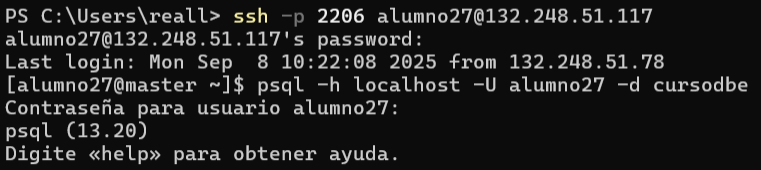
\includegraphics[width=1\linewidth]{Conexión a PostgreSQL.png}
    \caption{Conexión a PostgreSQL}
    \label{fig:placeholder}
\end{figure}

\subsection*{1.2 Identificación de la base de datos actual}
Se utiliza el comando \texttt{\textbackslash c} para verificar el nombre de la base de datos a la que estamos conectados actualmente.

\begin{figure}[h]
    \centering
    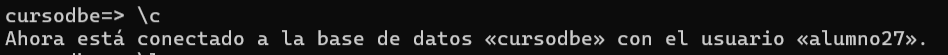
\includegraphics[width=1\linewidth]{Resultado del comando c.png}
    \caption{Resultado del comando \textbackslash c}
    \label{fig:placeholder}
\end{figure}

\subsection*{1.3 Listado de bases de datos}
Para listar todas las bases de datos administradas por el servidor, se ejecuta el comando correspondiente en \texttt{psql}.

\begin{figure}[h]
    \centering
    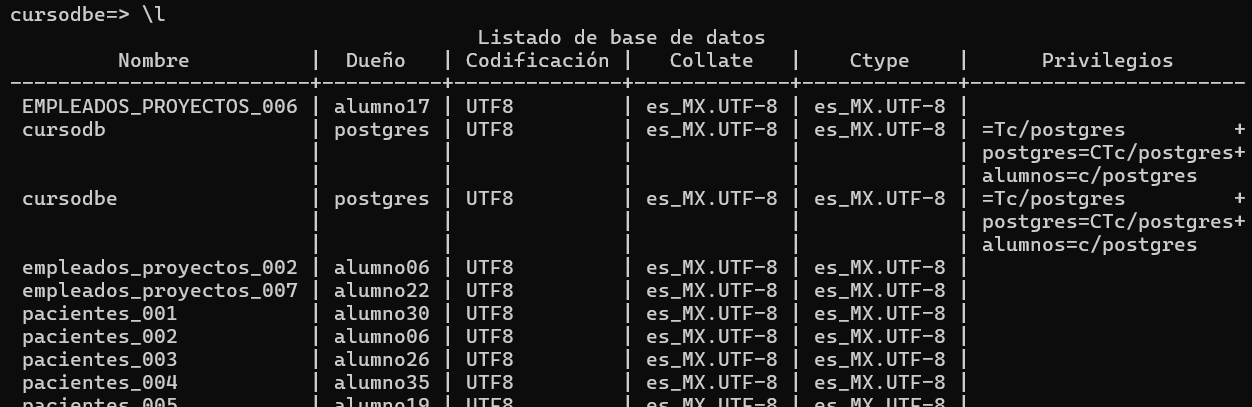
\includegraphics[width=1\linewidth]{Listado de bases de datos acortado (el original son 33 filas).png}
    \caption{Listado de bases de datos acortado (el original son 33 filas)}
    \label{fig:placeholder}
\end{figure}

\rule{\linewidth}{0.5mm}

\section*{Actividad 2: Consulta de la base de datos \texttt{cursodb}}
Se realizan consultas para inspeccionar los objetos dentro de las bases de datos \texttt{cursodb} y \texttt{proyectos}.

\subsection*{2.1 Listado de objetos en \texttt{cursodb}}
Se listan todas las tablas y objetos existentes en la base de datos \texttt{cursodb}.

\begin{figure}[h]
    \centering
    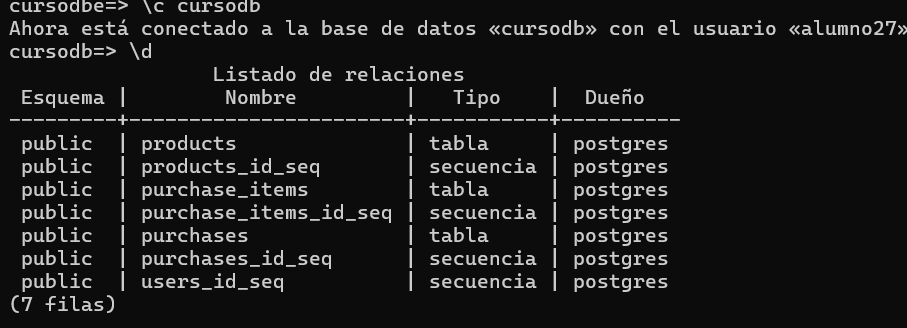
\includegraphics[width=1\linewidth]{Objetos en cursodb.png}
    \caption{Objetos en cursodb}
    \label{fig:placeholder}
\end{figure}

\subsection*{2.2 Detalles de las tablas}
Se despliegan detalles de \texttt{PURCHASES} y \texttt{PURCHASES\_ITEMS} para ver su estructura.

\begin{figure}[h]
    \centering
    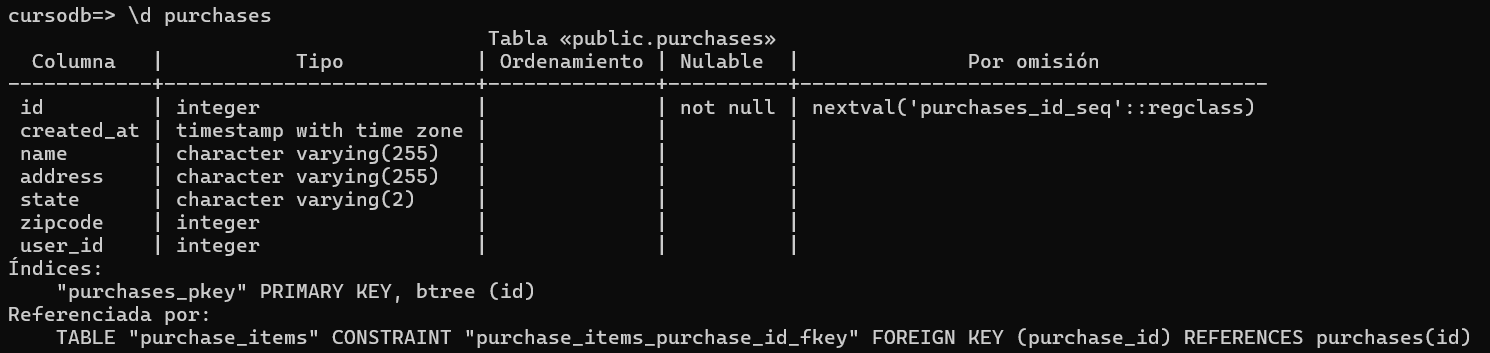
\includegraphics[width=0.95\linewidth]{Detalles de PURCHASES.png}
    \caption{Detalles de PURCHASES}
    \label{fig:placeholder}
\end{figure}
\newpage

\begin{figure}[h]
    \centering
    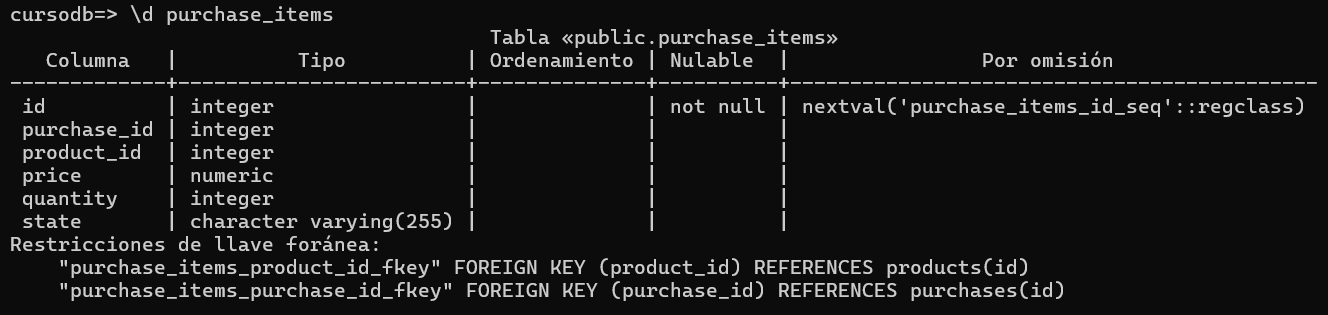
\includegraphics[width=1\linewidth]{Detalles de PURCHASES ITEMS.png}
    \caption{Detalles de PURCHASE ITEMS}
    \label{fig:placeholder}
\end{figure}

\subsection*{2.3 Cambio a la base de datos \texttt{proyectos} y listado de objetos}
Se realiza el cambio a la base de datos \texttt{proyectos} para explorarla y se listan los objetos de la base de datos.

\begin{figure}[h]
    \centering
    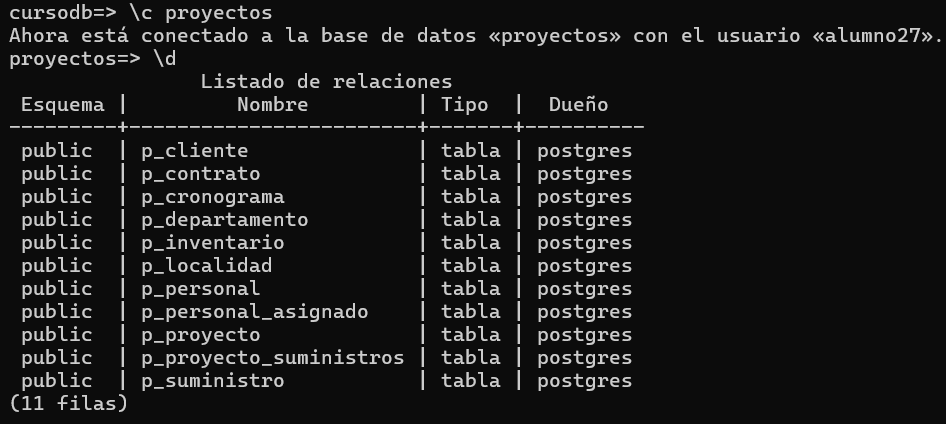
\includegraphics[width=1\linewidth]{Conexión a BD proyectos.png}
    \caption{Conexión a BD proyectos}
    \label{fig:placeholder}
\end{figure}

\rule{\linewidth}{0.5mm}

\section*{Actividad 3: Creación y ejecución de un script SQL}
En esta sección se crea, guarda y ejecuta un script de SQL para automatizar consultas.

\subsection*{3.1 Creación del script \texttt{lab\_03.sql}}
Se crea el archivo \texttt{lab\_03.sql} con el editor de texto vim, una mejora al clásico vi. Este script contiene los comandos para cambiar entre bases de datos y ejecutar consultas específicas.

\begin{figure}[h]
    \centering
    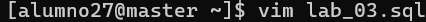
\includegraphics[width=0.5\linewidth]{lab03.png}
    \label{fig:placeholder}
\end{figure}
\begin{figure}[h]
    \centering
    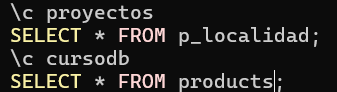
\includegraphics[width=0.5\linewidth]{lab_03 content.png}
    \caption{Contenido del script}
    \label{fig:placeholder}
\end{figure}


\subsection*{3.2 Ejecución del script}
Se ejecuta el script desde \texttt{psql} y se redirige la salida al archivo \texttt{resultado.txt}.

\begin{figure}[h]
    \centering
    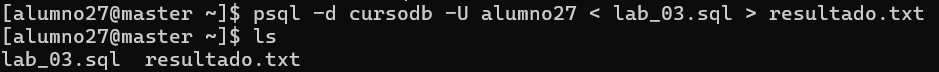
\includegraphics[width=0.92\linewidth]{Ejecución del script.png}
    \caption{Ejecución del script}
    \label{fig:placeholder}
\end{figure}

\begin{figure}[h]
    \centering
    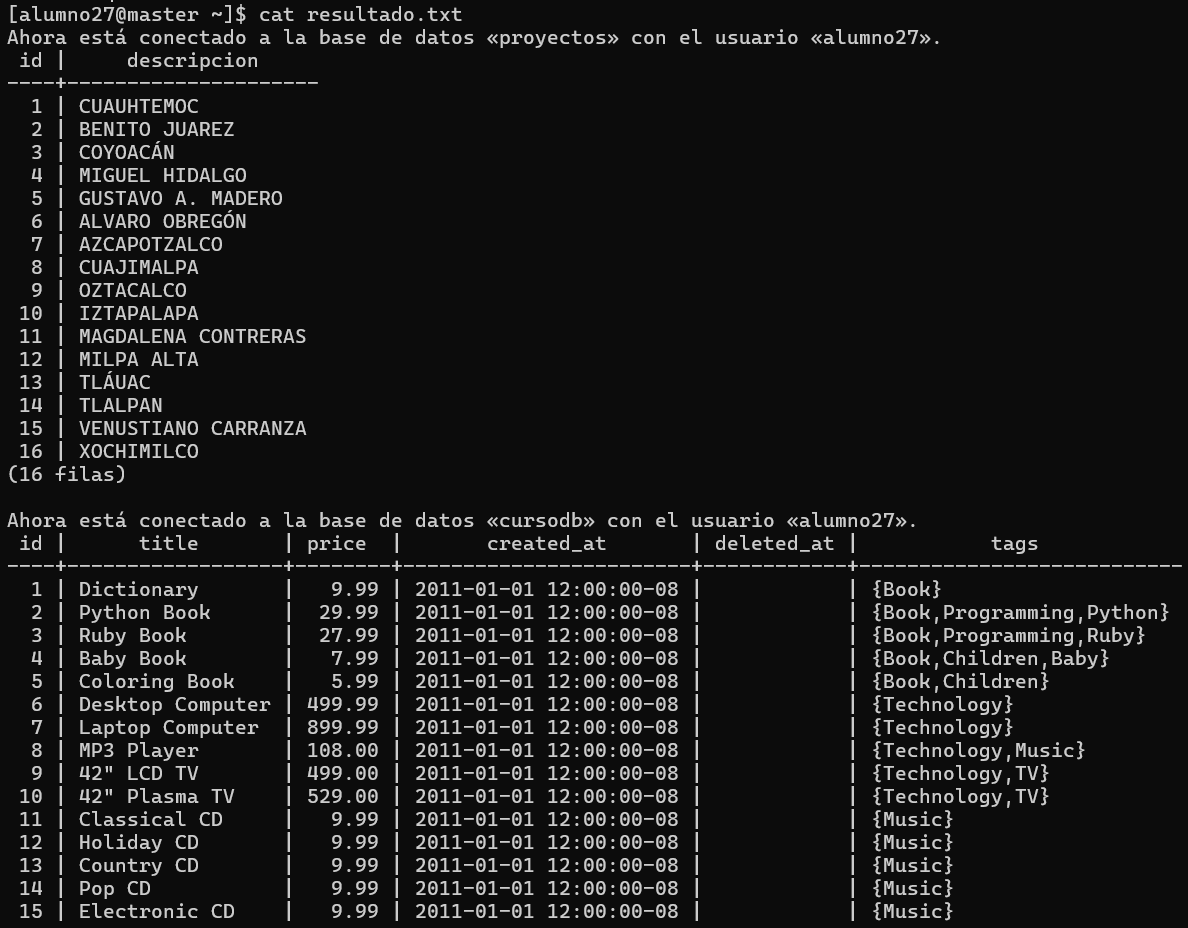
\includegraphics[width=0.9\linewidth]{Contenido de resultado txt.png}
    \caption{Contenido de resultado.txt (ligeramente recortado)}
    \label{fig:placeholder}
\end{figure}

\rule{\linewidth}{0.5mm}

\section*{Actividad 4: Creación de la base de datos \texttt{Reclusorios\_013}}
Se crea la base de datos \texttt{Reclusorios\_013} y todas las tablas correspondientes al modelo físico proporcionado.

\subsection*{4.1 Creación de la base de datos y sus tablas}
Se ejecuta el comando \texttt{CREATE DATABASE} para crear la base de datos. Se presenta el código SQL para la creación de las tablas, respetando las columnas, llaves primarias y foráneas indicadas en el diagrama.

\begin{figure}[h]
    \centering
    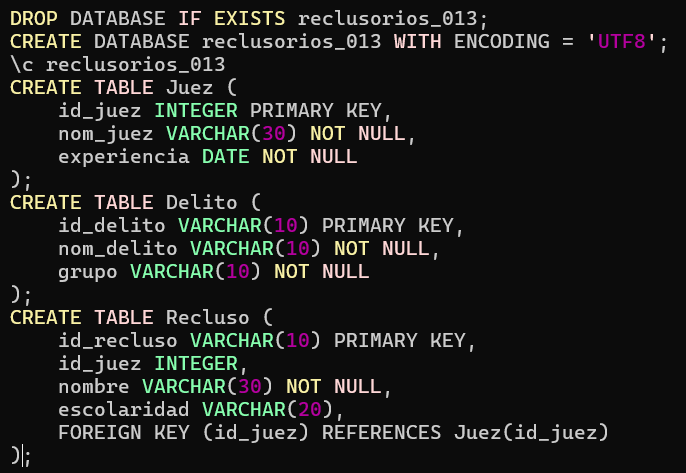
\includegraphics[width=0.8\linewidth]{Creación y conexión de BD Reclusorios.png}
    \caption{Creación de BD Reclusorios}
    \label{fig:placeholder}
\end{figure}

\textbf{Evidencia de la creación de las tablas y verificación final:}

\begin{figure}[h]
    \centering
    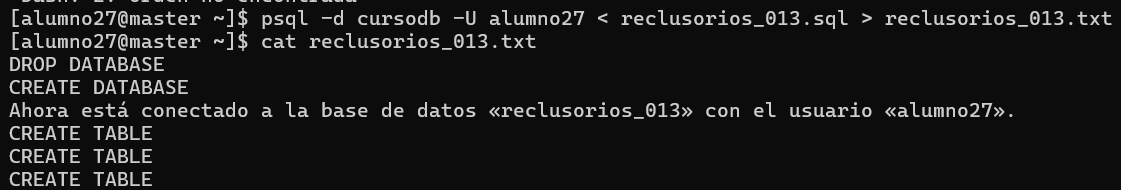
\includegraphics[width=1\linewidth]{Ejecución correcta (no errores).png}
    \caption{Ejecución correcta (no errores)}
    \label{fig:placeholder}
\end{figure}

\begin{figure}[h]
    \centering
    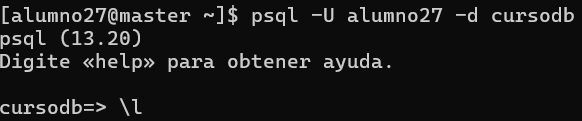
\includegraphics[width=1\linewidth]{h1.png}
    \label{fig:placeholder}
\end{figure}
\begin{figure}[h]
    \centering
    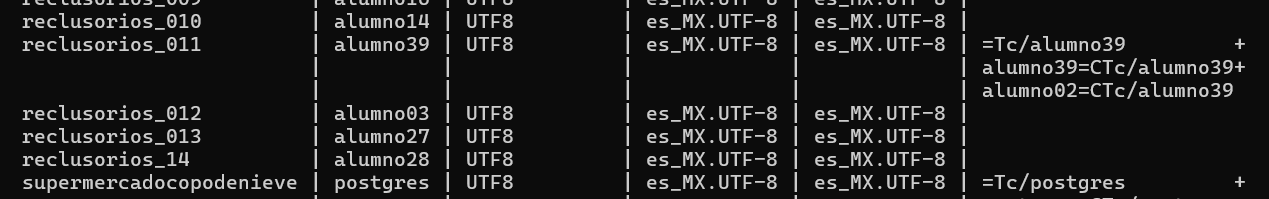
\includegraphics[width=1\linewidth]{Verificación formal (somos equipo 13 alumno 27).png}
    \caption{Verificación formal (somos equipo 13 alumno 27)}
    \label{fig:placeholder}
\end{figure}

\begin{figure}[h]
    \centering
    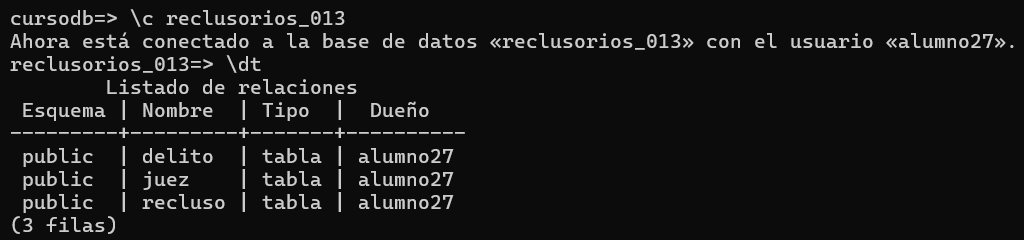
\includegraphics[width=1\linewidth]{Efectivamente está completa.png}
    \caption{Efectivamente está completa}
    \label{fig:placeholder}
\end{figure}

\section*{Actividad 5: Creación de la base de datos \texttt{Pacientes\_013}}
Se crea la base de datos \texttt{Pacientes\_013} y se definen sus tablas de acuerdo al modelo relacional especificado.

\subsection*{5.1 Creación de la base de datos}
Se ejecuta el comando para crear la base de datos \texttt{Pacientes\_013}, dado que el método de creación es análogo (uso de vim y ejecución, nos enfocaremos en mostrar que nuestro código es correcto).

\begin{figure}[h]
    \centering
    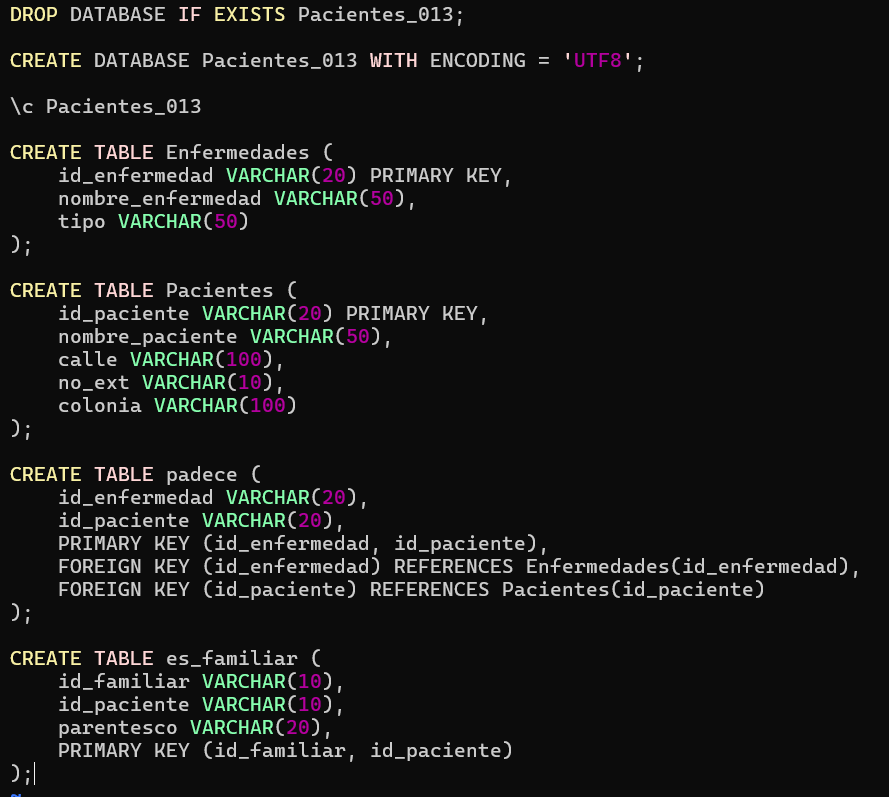
\includegraphics[width=0.5\linewidth]{Script para la creación de Pacientes_013.png}
    \caption{Primer script para la creación de Pacientes\_013}
    \label{fig:placeholder}
\end{figure}

\textbf{5.1.1 Identificación de fallo}
Se podría haber omitido esta subsubsección pero es enriquecedor ver estos errores. Según lo investigado es sugerible primero crear la base de datos, y en una ejecución aparte (creando otro script sql) crear las tablas, en muchas ocasiones puede fallar como lo que ha sucedido por lo cual por el resto de nuestras vidas usaremos esta convención.
\begin{figure}[h]
    \centering
    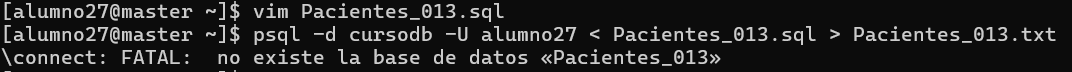
\includegraphics[width=1\linewidth]{Error5.1.png}
    \caption{Documentación de error en actividad 5.1}
    \label{fig:placeholder}
\end{figure}
\begin{figure}[h]
    \centering
    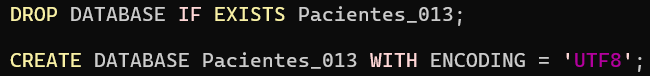
\includegraphics[width=0.5\linewidth]{Primer script para 5.1.png}
    \caption{Primer script para 5.1}
    \label{fig:placeholder}
\end{figure}
\begin{figure}[h]
    \centering
    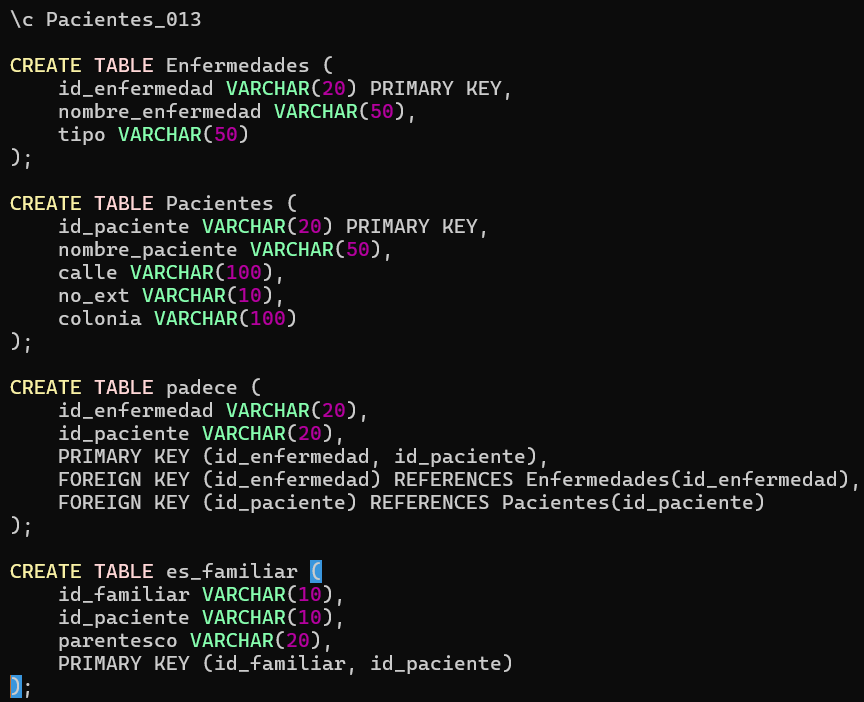
\includegraphics[width=0.9\linewidth]{Segundo script para 5.1.png}
    \caption{Segundo script para 5.1}
    \label{fig:placeholder}
\end{figure}

\subsection*{Verificación de la correcta creación de la base de datos.}
\begin{figure}[h]
    \centering
    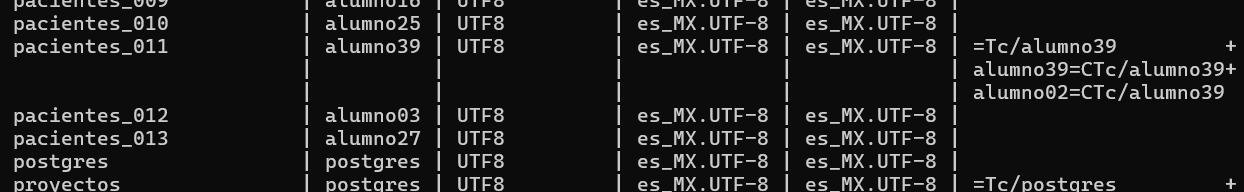
\includegraphics[width=1\linewidth]{Mi base de datos.png}
    \caption{Mi base de datos (Pacientes\_013)}
    \label{fig:placeholder}
\end{figure}

\begin{figure}[h]
    \centering
    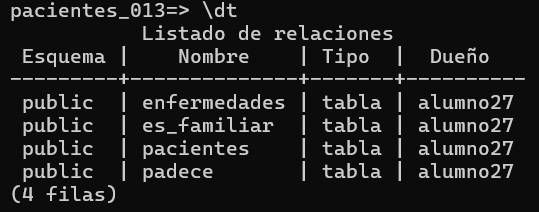
\includegraphics[width=0.7\linewidth]{Contenido de mi base de datos.png}
    \caption{Contenido base de datos Pacientes\_013}
    \label{fig:placeholder}
\end{figure}

\end{document}